
% ==============================================================================
% ==============================================================================
%
% HEADER
%
% ==============================================================================
% ==============================================================================

\documentclass{article}

\usepackage[T1]{fontenc}
\usepackage[utf8]{inputenc}
\usepackage[english]{babel}
\usepackage{graphicx}

\usepackage[
backend=biber,
%style=alphabetic,
%citestyle=authoryear
]{biblatex}

\usepackage{amssymb}
\usepackage{amsmath}
\usepackage{bm} % bold maths symbols
\usepackage{graphicx}
\usepackage{float}
\usepackage{hyperref}
\usepackage{algorithm}
\usepackage{algpseudocode}


\usepackage[a4paper, total={6in, 8in}]{geometry}


% ==============================================================================
% ==============================================================================
%
% DEFINITIONS
%
% ==============================================================================
% ==============================================================================
\addbibresource{cite.bib}


\renewcommand{\vec}[1]{\mathbf{#1}}
\renewcommand{\d}{\,\text{d}}


\newcommand{\A}{\mathcal{A}}
\newcommand{\E}{\mathcal{E}}
\newcommand{\F}{\mathcal{F}}
\renewcommand{\L}{\mathcal{L}}
\newcommand{\X}{\mathcal{X}}

\newcommand{\Enc}{\mathtt{Enc}}
\newcommand{\Dec}{\mathtt{Dec}}

\newcommand{\Oh}{\mathcal{O}}
\newcommand{\KL}[2]{\mathrm{KL}[\,#1\,\,||\,\,#2\,]}
\newcommand{\Exp}{\mathbb{E}}
\newcommand{\I}{\mathbb{I}}

\newcommand{\Hypos}{\mathcal{H}}
\newcommand{\Data}{\mathcal{D}}

\newcommand{\ImSpace}{\mathcal{X}}

\newcommand{\Reals}{\mathbb{R}}
\newcommand{\Ints}{\mathbb{Z}}
\newcommand{\Nats}{\mathbb{N}}

\newcommand{\Norm}[1]{\mathcal{N}\left( #1 \right)}
\newcommand{\Unif}[1]{\mathcal{U}\left( #1 \right)}
\newcommand{\Laplace}[1]{\mathcal{L}\left( #1 \right)}

% Bold maths symbols
\newcommand{\MU}{\boldsymbol\mu}
\newcommand{\SIGMA}{\boldsymbol\sigma}
\newcommand{\PSI}{\boldsymbol\psi}
\newcommand{\THETA}{\boldsymbol\theta}
\newcommand{\PHI}{\boldsymbol\phi}

\DeclareMathOperator*{\argmax}{arg\,max}
\DeclareMathOperator*{\argmin}{arg\,min}


\title{Compression without Quantization}
\author{Gergely Flamich}

% ==============================================================================
% ==============================================================================
%
% START OF THESIS
%
% ==============================================================================
% ==============================================================================

\begin{document}

\input{titlepage.tex}

% ==============================================================================
%
% DECLARATION
%
% ==============================================================================

\vspace{2cm}

\begin{center}
\Huge
\textbf{Declaration}
\end{center}

\vspace{1cm}

\large
\noindent I, Gergely Flamich of St John's College, being a candidate for the
MPhil in Machine Learning and Machine Intelligence, hereby declare that this
report and the work described in it are my own work, unaided except as may be
specified below, and that the report does not contain material that has
already been used to any substantial extent for a comparable purpose.


\vspace{2cm}

\large
\noindent
Wordcount: \textbf{16384} words

\newpage

% ==============================================================================
%
% ACKNOWLEDGEMENTS
%
% ==============================================================================

\vspace{2cm}

\begin{center}
\Huge
\textbf{Acknowledgements}
\end{center}

\vspace{1cm}



\newpage

% ==============================================================================
%
% ABSTRACT
%
% ==============================================================================

\begin{abstract}
  We provide an implementation of our proposed method written in \texttt{Tensorflow}
  \cite{tensorflow2015-whitepaper} and \texttt{Sonnet} \cite{sonnetblog},
  available on GitHub \footnotemark.
\end{abstract}

\footnotetext{https://github.com/gergely-flamich/miracle-compression}

\newpage

\tableofcontents

\newpage

% ==============================================================================
% ==============================================================================
%
% START OF CONTENTS
%
% ==============================================================================
% ==============================================================================

\section{Introduction}

High level description of every section

\subsection{Motivation}
- adaptive
- need for compression in a lot of new areas for which existing techniques might
not work well
lightfield cameras, 360 images / video, VR, video streams
- good handcrafted codecs are hard to design
- put the problem in a well-grounded mathematical framework, get theoretical guarantees

\subsubsection{Why Image Compression?}
\paragraph{}
Well studied problem, good literature availability, on handcrafted methods, NN
based methods and performance evaluation.

\subsubsection{Why Lossy?}
\paragraph{}
In lossless image compression we are limited by the true distribution of image
pixels in how much we can compress stuff.

In lossy compression we can make a huge saving, by only concentrating on details
that are perceptually important to the viewer.

\subsection{Our Goals}

Several metrics to optimise for:
- compression quality
- compression size
- compression time
- compressor size
- compressor power consumption
- robustness of compressor (i.e. resistance to errors / adversarial attacks)
- security / privacy of compression
- scalability: image size, image quality

\subsection{Our Contributions}
\paragraph{}

We present:
\begin{itemize}
\item a brief introduction to the technical background on neural-network
  based lossy image compression
\item a review of recent influential works in the area

\item a novel image compression algorithm trained on the CLIC 2018 dataset \cite{clic2018}

\item experiments and analysis of performance to confirm its theoretical properties
\end{itemize}

\subsection{Thesis Outline}
\paragraph{}



\section{Background}
\par
As compression is not a standard topic in machine learning, it will be useful to
first spend some time establishing the main concepts and familiarize ourselves
with the jargon. We first go through some notation that will be used throughout
this work. Then we go through a brief introduction to compression in general,
and lossy compression and transform coding in particular. Third, we examine the
motivating line of research to our project, the MDL framework, the bits-back
argument and MIRACLE. Although our work is inspired by and based on earlier
work, it differs from them in several significant ways. We will point out these
differences throughout.
\subsection{Notation and Basic Concepts}
\paragraph{}
It will be useful to clarify some of the notation throughout this work.
\begin{itemize}
\item Vectors will be denoted by boldface lowercase letters: $\vec{u}, \vec{x}, ...$
\item Matrices will be denoted by uppercase letters: $A, M, ...$
\item Probability mass functions will be denoted by uppercase letters: $P(x),
  Q(z), ...$
\item Probability density functions will be denoted by lowercase letters: $p(y),
  q(u), ...$
\item In general, exact/continuous values will be denoted by unannotated letters
  (e.g. $z_i, \vec{w}$), their quantized counterparts denoted by a hat
  ($\hat{z}_i, \vec{\hat{w}}$) and their approximate counterparts by a tilde
  ($\tilde{z}_i, \vec{\tilde{w}}$).
\item $\Exp_{p(x)}[f(x)]$ denotes the expected value of $f(x)$ with respect to
  the mass / density $p(x)$, i.e.:
  \[
    \Exp_{p(x)}[f(x)] = \int_\Omega f(x) \d p(x),
  \]
  where $\Omega$ is the sample space. As $\Omega$ will usually denote $\Reals^n$
  or will be understood from context, it will be omitted, and the integral will
  be rewritten as
  \[
    \Exp_{p(x)}[f(x)] = \int f(x)p(x) \d x.
  \]
\item $H[X]$ denotes the Shannon entropy of the random variable $X$. If $X$ is
  discrete, then it is defined as
  \[
    -\sum_{X=x}P(X=x)\log P(X=x).
  \]
  If it is continuous, then it will refer to the \textit{differential entropy}
  of $X$, namely
  \[
    -\int_{\X}\log p(x) \d p(x),
  \]
  where $\X$ denotes the support of $X$.
  \paragraph{Note:} we used the natural logarithm in our definition of entropy,
  and hence its units are \textbf{nats}. If we used the base 2 logarithm
  instead, the units would be \textbf{bits}.
\item $\KL{q(x)}{p(x)}$ denotes the Kullback-Leibler divergence between two
  distributions and is defined as
  \[
    \KL{q(x)}{p(x)} = \Exp_{q(x)}\left[\log\frac{q(x)}{p(x)}\right].
  \]
\item $I[X : Y]$ denotes the mutual information between random variables $X$ and
  $Y$ and is defined as
  \[
    I[X : Y] = \KL{p(x, y)}{p(x)p(y)},
  \]
  where $(X, Y) \sim p(x, y)$ and $p(x)$ and $p(y)$ denote the marginals.
\end{itemize}
\subsection{Image Compression}
\par
with 
\paragraph{Source Coding}
From a theoretical point of view, given some source $S$, a sender and a
receiver, compression may be described as the aim of the sender communicating an
arbitrary sequence $X_1, X_2, \hdots, X_n$ taken from $S$ to the receiver in as few bits
as possible such that the receiver may recover relevant information from the message.
If the receiver can always recover all the information from the message of the sender, we
call the algorithm \textbf{lossless}, otherwise we call it \textbf{lossy}. 
\par
At first it might seem non-sensical to allow for lossy compression, and in some
domains this is definitely true, e.g. in text compression. However, 
human's audio-visual perception is neither completely aligned with the range of
what can be digitally represented, nor does it always scale the same way. Hence,
there is a huge opportunity for compressing media in a lossy way by discarding
information with the change being imperceptible for a human observer, while
making huge gains in size reduction.
\paragraph{Lossy Compression}
As the medium of interest in lossy compression is generally assumed to be a
real-valued vectory $\vec{x} \in \Reals^N$, such as RGB pixel intensities in an
image or frequency coefficients in an audio file, the usual pipeline consists of 
an encoder $C \circ \Enc$ map a point $\vec{x} \in \Reals^N$ to a string of bits and a
decoder mapping from bitstrings to reconstruction $\vec{\hat{x}}$. The
factors of the encoder $\Enc$ and $C$ can be understood as a map from $\Reals^N$ to a
finite symbol set $\A$, called a \textbf{lossy encoder} and a map from $\A$ to a
string of bits called a \textbf{lossless code} \cite{goyal2001theoretical}.
We will examine both $\Enc$ and $C$ in more detail shortly. The decoder then can be
thought of as inverting the code first and then using an approximate inverse of
$\Enc$ to get the reconstruction $\vec{\hat{x}}$: $\Dec \circ C^{-1}$.
\par
It is important to be able to quantify
\begin{itemize}
\item the \textbf{distorsion} of the compressor: on average, how closely does
  $\vec{\hat{x}}$ resemble $\vec{x}$?
\item the \textbf{rate} of the compressor: on average, how many bits are
  required to communicate $\vec{x}$? We want this to be as low as possible of course.
\end{itemize}

\paragraph{Distorsion}
In order to measure ``closeness'' in the space of interest $\ImSpace$,
a distance metric $d(\cdot, \cdot): \ImSpace
\times \ImSpace \rightarrow \Reals$ is introduced. Then, the distortion $D$ is 
is defined as
\[
  D = \Exp_{p(\vec{\hat{x}})}[d(\vec{x}, \vec{\hat{x}})].
\]
A popular choice of $d$, across many domains of compression is the normalized $L_2$ metric
or MSE, defined as
\[
  d(\vec{x}, \vec{\hat{x}}) = \frac{1}{N} \sum_{i}^N (x_i - \hat{x}_i)^2, \quad
  \ImSpace = \Reals^N.
\]
It is a popular metric as it is simple, easy to implement and has nice
interpretations in both a Bayesian \cite{bishop2013pattern} and the MDL
(\cite{hinton1993keeping}, to be introduced in Section \ref{sec:mdl}) settings.
In the image compression setting, however, the MSE is problematic, since it is
optimizing for such metric does not necessarily translate to obtaining pleasant-looking
reconstructions \cite{zhao2015loss}, and hence more appropriate, so-called \textit{perceptual
  metrics} were developed. The ones relevant to our discussion are Peak
Signal-to-Noise Ratio (PSNR) \cite{psnr}, \cite{gupta2011modified} and the
Structural Similarity Index (SSIM) \cite{wang2004image} and its multiscale
version (MS-SSIM) \cite{msssim}. Crucially, these
two metrics are not only the most popular, but are also differentiable, which
means they lend themselves for gradient-based optimization.
PSNR is not a good metric \cite{girod1993s} \cite{eskicioglu1994image}.
% TODO --------------------------------------------------
\textbf{TODO: More discussion on metrics}

\paragraph{Rate}
We noted above that the code used after the lossy encoder is lossless. To
further elaborate, in virtually all cases it is an \textbf{entropy code}
\cite{goyal2001theoretical}. This means that we assume that each symbol
in the representation $\vec{z} = \Enc(\vec{x})$ has some probability mass
$P(z_i)$. A fundamental result by Shannon states that $\vec{z}$ may not be
encoded losslessly in fewer than $H[\vec{z}]$ nats
\cite{shannon1998mathematical}. Entropy codes, such as Huffman codes
\cite{huffman1952method} or Arithmetic Coding \cite{rissanen1981universal} can
get very close to this lower bound. We will coding methods further in Section
\ref{sec:mir_coding}. The rate (in nats) of the compression algorithm is defined
as the average number of nats required to code a single dimension of the input, i.e.
\[
  R = \frac{1}{N} H[\vec{z}].
\]
\paragraph{Transform Coding}
The issue with source coding is that coding $\vec{x}$ might have a lot of
dependencies across its dimensions. For images, this manifests on multiple
scales and semantic levels, e.g. a pixel being blue might indicate that most
pixels around it are blue as the scene is depicting the sky or a body of water;
a portrait of a face will also imply that eyes, a nose and mouth are probably
present, etc. Modelling and coding this dependence structure in very high
dimensions is highly non-trivial or perhaps even impossible, and hence we need
to make simplifying assumptions about it to proceed.
\par
\textit{Transform coding} attempts to solve the above problem by decomposing the
encoder function $\Enc = Q \circ T$ into a so-called \textbf{analysis transform}
$T$ and a \textbf{quantizer} $Q$. The idea is that to transform the input into a
domain, such that the dependencies between the dimensions are removed, and hence
they can be coded individually. The decoder inverts the steps of the encoder,
where the inverse operation of $T$ is called the \textbf{synthesis transform}
\cite{gupta2011modified}.
\par
In \textit{linear transform coding}, $T$ is an invertible linear trasformation,
such as a discrete cosine transformation (DCT), as it is in the case of JPEG
\cite{wallace1992jpeg}, or discrete wavelet transforms in JPEG 2000
\cite{rabbani2002overview}. While simple, fast and elegant, linear transform
coding has the key limitation that it can only at most remove correlations (i.e.
first-order dependencies), and this can severly limit its efficiency
\cite{balle2016endtrans}. Instead, \cite{balle2016endtrans} propose a method for
\textit{non-linear transform coding}, where $T$ is replaced by a highly
non-linear transformation, and its inverse is now replaced by an approximate
inverse, which is a separate non-linear transformation. Both $T$ and its
approximate inverse are learnt, and the authors show that with a more
complicated transformation they can easily surpass the performance of the much
more fine-tuned JPEG codecs.
\par
Our work also falls into this line of research, although with signifcant
differences, which will be pointed out later.
\subsection{The MDL principle and the Bits-Back Argument}
\label{sec:mdl}
\paragraph{MDL Principle} 
Our approach is based on the Minimum Description Length (MDL) Principle
\cite{rissanen1986stochastic}. In essence, it is a formalization of Occam's
Razor, i.e. the simplest model that describes the data well is the best model of
the data \cite{grünwald2007minimum}. Here, ``simple'' and ``well'' need to be
defined, and these definitions are precisely what the MDL principle gives us.
Informally, it asserts that given a class of hypotheses $\Hypos$ (e.g. a certain
statistical model and its parameters) and some data $\Data$, if a particular
hypothesis $H \in \Hypos$ can be described with at most $L(H)$ bits and the using the
hypothesis the data can be described with at most $L(\Data \mid H)$ bits, then the
minimum description length of the data is
\begin{equation}
\label{eq:min_desc_princ}
  L = \min_{H \in \Hypos}\{ L(H) + L(\Data \mid H) \},
\end{equation}
and the best hypothesis is the $H$ that minimizes the above quantity.
\par
Crucially, the MDL principle can thus be interpreted as telling us that
\textbf{the best model of the data is the one that compresses it the most}.
This makes Eq \ref{eq:min_desc_princ} a very appealing learning objective for
optimization-based compression methods, ours included.
Below, we briefly review how this has been applied so far and how it translates
to our case.
\paragraph{Bits-Back Argument}
First, we begin with the bits-back argument, introduced in
\cite{hinton1993keeping}, which is a direct application of the above. The main
goal of this work was to develop a regularisation technique for neural networks
by framing the training of a neural network as a communication problem, where
the training input and the fixed network architecture is public, but the weights,
the network's output given a particular input, and the training targets are
only available to the sender, and the task is to communicate the
\textit{training targets} with minimal bits.
\par
Concretely, they train a Bayesian Neural Network, by equipping the weights
$\vec{w}$ with a prior $p_\theta(\vec{w})$ and a posterior $q_\phi(\vec{w})$
(parameterized by $\theta$ and $\phi$, respectively) and maximize
the \textit{evidence lower bound} (ELBO) given a likelihood $p(\Data \mid \vec{w})$:
\begin{equation}
  \label{eq:elbo_target}
  \Exp_{q_\phi}[\log p(\Data \mid \vec{w})] - \KL{q_{\phi}}{p_{\theta}}.
\end{equation}
Given a sufficiently finely quantized likelihood, the minimum description length
of the data given this model is $\Exp_{q_\phi}[-\log p(\Data \mid \vec{w})]$
\cite{shannon1998mathematical}, and hence the first term in Eq
\ref{eq:elbo_target} corresponds to $-L(\Data \mid H)$. In their work then,
\cite{hinton1993keeping} show that the second term in Eq \ref{eq:elbo_target}
is equal to $-L(H)$, which establishes a link between the variational training
objective of the BNN and the MDL principle.
\par
To do this, the encoder
\begin{enumerate}
\item trains the neural network, optimising Eq \ref{eq:elbo_target}.
\item draws a random sample $\vec{\hat{w}} \sim q_{\phi}(\vec{w})$. This
  represents a message of $\Exp_{q_\theta}[- \log q_\phi]$ nats.
\item $\vec{\hat{w}}$ is then used to calculate the residuals $\vec{r}$ between
  the network's output and the targets.
\item $\vec{r}$ is coded with $\vec{\hat{w}}$ and then $\vec{\hat{w}}$ is coded
  using its prior $p_\theta$. The total length of the message is hence $\Exp_{q_\phi}[-\log
  p(\Data \mid \vec{\hat{w}})] + \Exp_{q_\phi}[-\log p_{\theta}]$.
\end{enumerate}
Once everything has been communicated, the decoder can recover the true training
targets, but then they can also run the same training algorithm that the encoder
used to then recover the posterior $q_\phi$. This means that the code of
$\vec{\hat{w}}$ is ``free bits'' in the sense that the decoder can recover them
exactly given what they already have. 
Hence, the whole cost of drawing $\vec{\hat{w}}$ should be
subtracted from the original cost, yielding
$\Exp_{q_\phi}[-\log p_{\theta}] - \Exp_{q_\phi}[-\log q_{\phi}] =
\KL{q_{\phi}}{p_\theta}$ nats. This ``recovery'' is the namesake for the
bits-back argument.
\paragraph{MIRACLE}
Inspired by the above idea, \cite{havasi2018minimal} asked a natural question:
\textit{is it possible to communicate only the weights of a network at
  bits-back efficiency?}
\par
If the above were true, it would give a method for compressing neural networks
rather efficiently. It is clear that the coding must be different than it was in
\cite{hinton1993keeping}, as their method focused on the regularisation aspect
of the KL-divergence and is very inefficient for actual communication of the
model parameters.
\par
A second, important question that arises in conjunction with the first, natural
for compression algorithms:
\textit{is it possible trade off accuracy of a fixed neural network architecture
  for better compression rates, and vice versa?}
\par
Luckily, the answer to both of the above questions is yes, and we shall begin by
addressing the latter first. Fix a network architecture, and some data
likelihood given a weight set $p(\Data \mid \vec{\hat{w}})$. Akin to
\cite{hinton1993keeping}, we will actually train a BNN with weight prior
$p(\vec{w})$ and posterior $q(\vec{w})$. Then, given a budget of $C$ nats, we
hope to maximize the following constrained objective:
\begin{equation}
\label{eq:miracle_hard_train_target}
\Exp_{q_\phi}[\log p(\Data \mid \vec{w})] \quad \text{subject to }
\KL{q_{\phi}}{p_{\theta}} < C.
\end{equation}
We can rewrite Eq \ref{eq:miracle_hard_train_target} as its Lagranagian
relaxation under the KKT conditions \cite{karush2014minima},
\cite{kuhn2014nonlinear}, \cite{higgins2017beta} and get:
\[
  \F(\theta, \phi, \beta, \Data, \vec{\hat{w}}) = 
  \Exp_{q_\phi}[\log p(\Data \mid \vec{\hat{w}})] - \beta (\KL{q_{\phi}}{p_{\theta}} - C).
\]
By the KKT conditions if $C \geq 0$ then $\beta \geq 0$, hence discarding the last
term in the above equation will provide a lower bound for it:
\begin{equation}
\label{eq:miracle_train_target}
\F(\theta, \phi, \beta, \Data, \vec{\hat{w}}) \geq
\L(\theta, \phi, \beta \Data, \vec{\hat{w}}) =
\Exp_{q_\phi}[\log p(\Data \mid \vec{\hat{w}})] - \beta \KL{q_{\phi}}{p_{\theta}}.
\end{equation}
Notice, that this is the same as Eq \ref{eq:elbo_target}, but with the addition of
the parameter $\beta$ that will control the regularisation term and eventually
the compression cost of the weights. It is also intimately related to the
training target of $\beta$-VAEs \cite{higgins2017beta}, except for where they
regularise the distributions of activations on a stochastic layer, here the
regularisation is for the distributions of weights. 
\par
Now, to answer the first question, we first need to establish the right setting
for the task, which will be another communications problem.
Concretely, given a dataset $\Data$ sampled from a distribution $p(D)$, and
$q_\phi(\vec{w})$, our trained weight posterior for a given $\beta$, what are
the bounds on the minimum description length for the posterior $L(q_{\phi})$?
\par
Under some mild assumptions, it can be shown \cite{harsha2007communication} that
in fact
\[
  \Exp_{p(D)}[L(q_{\phi})] \geq \Exp_{p(D)}[\KL{q_{\phi}}{p_{\theta}}],
\]
i.e. in this probabilistic setting bits-back efficiency is the best we can hope
for. Now, if we make the further assumption that the sender and the receiver are
allowed to \textit{share a source of randomness} (e.g. a random number generator
and a seed for it), then a rather tight upper bound can also be derived, also
due to \cite{harsha2007communication}:
\begin{equation}
\label{eq:miracle_ub}
  \Exp_{p(D)}[L(q_{\phi})] \leq I[\Data : \vec{w}] + 2 \log \left( I[\Data :
    \vec{w}] + 1 \right) + \Oh(1)
\end{equation}
where $I[D : \vec{w}] = \Exp_{p(D)}[\KL{q_{\phi}}{p_{\theta}}]$ is the
mutual information between the distribution of datasets and the weights.
\paragraph{Note:} Hence, tuning $\beta$ in \ref{eq:miracle_train_target}
\textit{directly} controls the rate of the compression algorithm.
\par
Eq \ref{eq:miracle_ub} is proven by exposing an algorithm that achieves the
postualted coding efficiency, an adaptive rejection sampling algorithm, which we
detail in the Appendix A. This turns out to be infeasible in the case of
MIRACLE, and instead the authors propose an importance sampling-based
approximate sampling algorithm, which is also discussed in further detail in
Appendix A. They are important, as we have used both in our project.

\paragraph{Our method} Our project is based upon the simple observation, that
the MIRACLE framework may be utilised for compression of any data where in our
model a public prior distribution $p_{\theta}$ and a learned $q_{\phi}$ is
available and we are allowed to share a source of randomness. We have already
noted the extreme similarity of the original BNN training objective to that of
the $\beta$-VAE \cite{higgins2017beta}, and indeed they are precisely the model
that we shall use for the compression of images in our case.

% ==============================================================================
% ==============================================================================
%
% Related work
%
% ==============================================================================
% ==============================================================================

\section{Related Work}
\par
Here we give a brief overview of the history of using machine learning for image
compression. Then, we focus on recent advances in lossy image compression and
describe and compare their methods to each other as well as ours.
\subsection{Machine Learning-based Image Compression}
\par

First attempt by \cite{bottou1998high} DjVu focused on segmenting foreground and
background in magazines and using K-means clustering to analize and code the
background.

Neural network based image compression has been theorized about for a long time
now \cite{mougeot1991image} \cite{jiang1999image} 
\cite{toderici2015variable} focused only 32x32 thumbnails
Image reconstruction through compressive representations \cite{denton2015deep},
\cite{gregor2015draw}

\subsection{Comparison of Recent Works}
\label{sec:lit_comparison}
\par

There have been several recent advances in neural network-based compression
techniques, most notably \cite{toderici2015variable}, \cite{balle2016end},
\cite{toderici2017full}, \cite{theis2017lossy}, \cite{rippel2017real},
\cite{balle2018variational}, \cite{johnston2018cvpr}, \cite{mentzer2018cvpr}. 
An interesting commonality between these approaches is that there is very little
commonality between them, for a multidue of reasons, on which we hope to shed
some lite in this section. Instead of analyzing them in a historical order, we
will instead go through the compression pipeline and compare them head-to-head
in each compartment separately. 
\subsubsection{Datasets and Input Pipelines}
\par
Somewhat surprisingly it appears that there is no canonical dataset (yet) for
the task at hand, namely a set of high-resolution, variable-sized losslessly
encoded colour images,
although CLIC \cite{clic2018} seems to be an emerging one. Perhaps the reason is
that generally in other domains, such as image-based classification cropping and
rescaling images can effectively side-step the need to deal with variable-sized
images. However, when it comes to compression, if we hope to build anything
useful, we must account for this.
\par
On the other hand most authors have used the Kodak dataset \cite{kodakdataset}
for testing / reporting results.
\begin{itemize}
\item \cite{balle2016end} trained on 6507 images, selected from ImageNet
  \cite{deng2009imagenet}. They removed images with excessive saturation and
  since their method is based on dithering, they added unifrom noise to the
  remaining images to imitate the noise introduced by quantization. Finally,
  they downsampled and cropped images to be $256 \times 256$ pixels in size.
  They only kept images whise resampling factor was 0.75 or less, in order to
  avoid high frequency noise.
\item \cite{toderici2017full}
  used two datasets, first the one they described in \cite{toderici2015variable}
  and the second one (they call the ``High Entropy'' dataset) was created by
  first scraping 6 million images from the web, then resizing them to $1280
  \times 720$ pixels. Then, they decomposed these into $32 \times 32$ pixel
  tiles and selected the 100 tiles from each with the worst compression ratio under
  the PNG algorithm.
\item \cite{theis2017lossy} used 434 high resolution images from \url{flickr.com}
  under the creative commons license. As \texttt{flickr} store its images as
  JPEGs, they downsampled all images to be below $1536 \times 1536$ in
  resolution and saved them as PNGs in order to reduce the effects of the lossy
  compression. Then, they extracted several $128 \times 128$ patches from each
  image and trained on those.
\item \cite{rippel2017real} took images from the Yahoo Flickr Creative Commons
  100 Million dataset, with $128 \times 128$ patches randomly sampled from the
  images. They do not state whether they used the whole dataset or just a
  subset, neither do they describe further preprocessing steps.
\item \cite{balle2018variational} scraped $\approx$ 1 million colour JPEG images
  of dimensions at most $3000 \times 5000$. They filtered out images with
  excessive saturation similarly to \cite{balle2016end}. They also
  downsampled images by random factors such that the image's height and width
  stayed above 640 and 1200 pixels, respectively. Finally, they use several
  randomly cropped $256 \times 256$ pixel patches extracted from each image.
% \item \cite{johnston2018cvpr} similarly to the ``High Entropy'' dataset in
%   \cite{toderici2017full}, they scrape 6 million JPEG images from the web and
%   extract $128 \times 128$ patches from them to train on.
% \item \cite{mentzer2018cvpr} train on the ILSVRC2012 ImageNet dataset 
%   \cite{russakovsky2015imagenet}. They take extract $160 \times 160$ pixel image
%   patches and randomly flipped them.
\end{itemize}

\subsubsection{Architectures}
\par
This is the most diverse aspect of recent approaches, and so we will only
discuss them on a very high level. We took inspiration from most of these papers
as well as others, these will be emphasized in Section \ref{sec:our_method}.

\begin{itemize}
\item \cite{balle2016end} Build a relatively shallow autoencoder (5 layers).
  There are several non-standard techniques they use, however. Firstly, their
  architecture is fully convolutional, i.e. all linear transformations in their
  network are convolutions in the encoder and deconvolutions in the decoder.
  They also downsample after the linear transformations, however, this is not
  elaborated upon in the work, neither is whether they padded the convolutions
  and if so how.
  This leads to the very natural consequence that their latent space and hence
  the code of an image grows with its size. Secondly they do not use any
  standard non-linearity or batch normalization. Instead, they propose their own
  activation function, custom tailored for image compression. These
  non-linearities are a form of adaptive local gain control for the images,
  called Generalized Divisive Normalization (GDN). At the $k$th layer for
  channel $i$ at position $(m, n)$, for input $w_i^{(k)}(m, n)$, the GDN
  transform is defined as
  \begin{equation}
    \label{eq:gdn_def}
    u_i^{(k + 1)}(m, n) = \frac{w_i^{(k)}(m, n)}{
      \left( \beta_{k, i} + \sum_j \gamma_{k, i, j}
        \left( w_{j}^{(k)}(m, n)\right)^2 \right)}.
  \end{equation}
  Its approximate inverse, IGDN for input $\hat{u}_i^{(k)}(m, n)$ is defined as
  \begin{equation}
    \label{eq:igdn_def}
    \hat{w}_i^{(k)}(m, n) = \hat{u}_i^{(k)}(m, n) \cdot \left(
      \hat{\beta}_{k, i} + \sum_{j} \hat{\gamma}_{k, i, j} \left(
      \hat{u}_j^{(k)}(m, n)\right)^2 \right)^{\frac{1}{2}}.
  \end{equation}
  Here, the set $\beta_{k, i}, \gamma_{i, j, k}, \hat{\beta_{k, i}},
  \hat{\gamma_{i, j, k}}$ are learned during training and fixed at test time.
  
\item \cite{toderici2017full}
\item \cite{theis2017lossy} define a Compressive Autoencoder (CAE) as a regular
  autoencoder with the quantization step between the encoding and decoding step.
  (In this sense, the architectures of \cite{balle2016end} and
  \cite{balle2018variational} are also CAEs.) They mirror pad the input first
  and then they follow it up by a deep, fully convolutional, residual
  architecture \cite{he2016deep}. They use valid convolutions and downsample by
  using a stride of 2. Between convolutions they use leaky ReLUs as
  nonlinearities, which are defined as 
  \[
    f_\alpha(x) = \max\{x, \alpha x\}, \quad \alpha \in [0, 1].
  \]
  The decoder mirrors the encoder. When upsampling is required, they use what
  they term \textit{subpixel} convolutions, where they perform a regular
  convolution operation with an increased number of filters, and then reshape
  the resulting tensor into one with larger spatial extent but fewer channels.
\item \cite{rippel2017real} use a fully convolutional encoder/decoder pair,
  downscaling between convolutions. They also add in an additional residual
  connection from every layer to the last, summing at the end. They call this
  \textit{pyramidal decomposition} and \textit{interscale alignment}, with the
  rationale behind it being that the residual connections extract features at
  different scales, and so the latent representations can take advantage of this.
\item \cite{balle2018variational} extend the architecture presented in
  \cite{balle2016end}. In particular, the encoder and decoder remain the same,
  and they add an additional stochastic layer on top of the architecture.
  However, it is important to note, that this is not a hierarchical VAE, it
  resembles instead a probabilistic ladder network \cite{sonderby2016train}.
  The layers leading to the second level are more standard, it is still fully
  convlutional with downsampling after convolutions, however, instead of GDN
  they use ReLUs.
  \par
  A slightly strange
  design choice on their part is since they will wish to force the second stage
  activations to be positive (it will be predicting a scale parameter), instead
  of using an exponential or softplus ($\log (1 + \exp\{x\})$) activation at the
  end, they take the absolute value of the input to the first layer, and rely on
  the ReLUs never giving negative values. We are not sure if this was meant to
  be a computational saving, as taking absolute values is certainly cheaper then
  either of the aforementioned standard ways of forcing positive values, or it
  if it gave better results.
\end{itemize}

\subsubsection{Quantization}
\label{sec:comp_quant}
\par
As all methods surveyed here are trained using gradient-based methods, a crucial
question that needs to be answered is how they dealt with the issue of
quantization. This is because encoding an image, quantizing the result and then
decoding the dequantized representation is problematic as the quantization step
yields 0 derivatives almost everywhere. There are two particular items that need
to be circumvented: first, the quantization operation itself, and second, the
rate estimator $H[P(\vec{z})]$. In the next section, we will see how our method
suffers from neither of these issues, as we forego the quantization step altogether.
\begin{itemize}
\item
  \textbf{Quantization }
  \cite{balle2016end} Quantize the output of their encoder $\vec{z}$ as
  \[
    \hat{z}_i = [z_i], 
  \]
  where $[\cdot]$ denotes the rounding operation. They model this 
  quantization error as dither, i.e. they replace their quantized latents
  $\hat{z}_i$ by
  \[
    \tilde{z}_i = z_i + \delta z_i, \quad z_i \sim \Unif{0, 1}. 
  \]
  \par \textbf{Rate }
  To model the rate, they also require to learn a distribution over the
  $\tilde{z}_i$s. They assume that the latents are independent, and hence they
  can model the the joint as a fully factorized distribution. They use linear
  splines to do this, whose parameters $\psi^{(i)}$ they update separately every
  $10^6$ iterations using SGD to maximize its log likelihood on the latents.

\item \cite{toderici2017full}
\item
  \textbf{Quantization }
  \cite{theis2017lossy} also use rounding as their quantization step.
  However, instead of using uniform noise to model the quantization error, they
  simply replace the derivative of the rounding operation in the backpropagation
  chain by the constant function 1:
  \[
    \frac{d}{d y} [y] = 1.
  \]
  This is a smooth approximation of rounding and they report that empirically it
  gave good results. However, as quantization itself creates an important
  bottleneck in the flow of information, it is key that only the derivative is
  replaced and not the operation itself.
  \par \textbf{Rate }
  They note that
  \[
    P(\vec{z}) = \int_{[-\frac{1}{2}, \frac{1}{2})^M} q(\vec{z} + \vec{u}) \d \vec{u}
  \]
  for some appropriate density $q$,
  where the integral is taken over the centered $M$ dimensional hypercube.
  Then, they replace the the rate estimator with an upper bound using Jensen's
  inequality:
  \[
    -\log_2P(\vec{z}) = -\log_2\int_{[-\frac{1}{2}, \frac{1}{2})^M} q(\vec{z} +
    \vec{u}) \d \vec{u} \leq -\int_{[-\frac{1}{2}, \frac{1}{2})^M} \log_2q(\vec{z} +
    \vec{u}) \d \vec{u}.
  \]
  This upper bound is now differentiable. They pick a Gaussian Scale Mixtures for
  $q$, with $s = 6$ components, with the mixing proportions fixed across spatial
  dimensions, which gives the negative log likelihood
  \[
    -\log_2 q(\vec{z} + \vec{u}) =
    \sum_{i, j, k} \log_2 \sum_s \pi_{k, s} \Norm{z_{k,i,j} + u_{k, i, j} \mid
    0, \sigma_{k, s}^2},
  \]
  where $i,j$ iterate through the spatial dimensions and $k$ indexes the filters.
  
\item
  \textbf{Quantiazation }
  \cite{rippel2017real} use the following formula:
  \[
    \hat{z}_i = \frac{1}{2^B}\left\lceil 2^Bz_i \right\rceil
  \]
  with $B = 6$. For $B = 1$ this gives a similar error as rounding, and as $B$
  is increased, the quantization gets finer. They do not report how they
  circumvented the non-differentiability of the quantization step, however, they
  do cite both \cite{balle2016end} and \cite{theis2017lossy}, so our guess is
  that they used a method from one of these papers.

  \textbf{Rate } they do not train for the rate-distrotion trade-off directly
  and in particular omit the rate estimator from the loss. Hence there was no
  need for them to approximate it to make it differentiable.
\item
  \textbf{Quantization }
  \cite{balle2018variational} the quantization scheme remains the same as in
  \cite{balle2016end}, extended to the second stochastic layer as well.

  \textbf{Rate } 
  As for the rate, they us a non-parametric, fully factorized prior for the
  second stage:
  \[
    p(\vec{\tilde{z}}^{(2)} \mid \psi) =
    \prod_i \left(  p\left(\tilde{z}^{(2)}_i \mid \psi_i\right) *
      \Unif{-\frac{1}{2}, -\frac{1}{2}\right)}.
  \]
  Then, they model the first stage as dithered zero-mean Gaussians with variable
  scale depending on the second stage, thereby relaxing the initial independence
  assumption on the latent space to a more general \textit{conditional
    indepenence} assumption \cite{bishop1998latent}:
  \[
    p(\vec{\tilde{z}}^{(1)} \mid \vec{\tilde{z}}^{(2)}) = 
    \prod_i \left(  \Norm{\tilde{z}^{(1)}_i \mid 0, \tilde{\sigma}^2_i\right)*
      \Unif{-\frac{1}{2}, -\frac{1}{2}}}.
  \]
\end{itemize}

Crucially, the rate term in our optimization objective is different from
previous approaches, in that in previous approaches the distribution of the
codewords was estimated separately. In our case, however, it is an integral part
of the optimization process.

In \cite{theis2017lossy}, they demonstrate that it is precisely the quantization
step that introduces the noisy artifacts into the image, and not the
reconstruction procedure. This is fundamentally different from our case, where
the majority of the quality degradation comes from the fact that VAEs generally
produce blurry reconstructions.

\subsubsection{Coding}
\par
Another important part of the examined methods is the coding. In particular, an
interesting caveat of entropy codes is that they tend to perform slightly worse
than the predicted rate, due to neglected constant factors in the algorithm
\cite{rissanen1981universal}. Hence, it is always more informative to present
results where the actual coding has been performed and not just the theoretical
rate reported. All examined works have implemented their own coding algorithms,
and we briefly review them here.
\begin{itemize}
\item \cite{balle2016end} Context adaptive binary arithmetic coding (CABAC),
  they supply new information in raster-scan order, which means it does not
  improve much over non-adaptive coding, but there might be potential
\item \cite{toderici2017full}
\item \cite{theis2017lossy} used their estimated probabilities $q(\vec{z})$ and
  used an off-the-shelf publicly available range coder to compress their latents.
\item \cite{rippel2017real} treat each bit of their $B$-bit precision quantized
  representations individually, because they want to utilize the sparsity of
  more significant bits. They train a separate binary classifier to predict
  probabilities for each individual bit based on a set of features (they call
  it a \textit{context}) to use in an adaptive arithmetic coder. They further
  add a regularizing term during training based on the codelength of a batch to
  match a length target. This is to encourage sparsity for high-resolution, but
  low entropy images and a longer codelength for low resolution but high entropy
  images.
\item \cite{balle2018variational} use a non-adaptive arithmetic coder as their
  entropy code. As they have two stochastic levels, with the
  first depending on the second, they have to code them sequentially. For the
  second level, they get their frequency estimates for $\vec{\hat{z}}^{(2)}$
  from the non-parametric prior:
  \[
    p(\hat{z}^{(2)}_i) =
    \int_{\hat{z}^{(2)}_i-\frac{1}{2}}^{\hat{z}^{(2)}_i+\frac{1}{2}}p(\tilde{z}_i \mid \psi_i) \d \tilde{z}_i.
  \]
  Then, on the first level, their probaibilities are given by:
  \[
    p(\hat{z}^{(1)} \mid \tilde{z}^{(2)}) = p(\hat{z}^{(1)} \mid
    \tilde{\sigma}^2_i) = 
    \int_{\hat{z}^{(1)}_i-\frac{1}{2}}^{\hat{z}^{(1)}_i + \frac{1}{2}}\Norm{\tilde{z}_i \mid 0, \tilde{\sigma}^2_i} \d \tilde{z}_i.
  \]

\end{itemize}

\subsubsection{Training}
\par
\begin{itemize}
\item \cite{balle2016end} Set out to train for the rate-distrotion trade-off
  directly, i.e.
  \[
    L = H[\vec{\hat{z}}] + \beta \Exp[d(\vec{x}, \vec{\hat{x}})],
  \]
  where the expectation is taken over training batches.
  As this is a non-differentiable loss function due to the quantization, they
  replace the discrete entropy term with a differential entropy term:
  \[
   L = \Exp\left[ -\sum_i \log_2 p(z_i + \delta z_i \mid \psi^{(i)}) +
                     \beta d(\vec{x}, \vec{\hat{x}})\right].
  \]
  \par Since they use MSE as the distance metric, they note that their
  architecture could be considered as an, albeit somewhat
  strange, VAE with Gaussian likelihood
  \[
    p(\vec{x} \mid \vec{\tilde{z}}, \beta) =
    \Norm{\vec{x} \mid \vec{\hat{x}}, (2\beta)^{-1}\vec{1}},
  \]
  mean-field prior
  \[
    p(\vec{\tilde{z}} \mid \psi^{1}, \hdots, \psi^{N}) =
    \prod_i p(\tilde{z}_i \mid \psi^{(i)})
  \]
  and mean-field posterior
  \[
    q(\vec{\tilde{z}} \mid \vec{x}) =
    \prod_i \Unif{\tilde{z}_i \mid z_i, 1},
  \]
  where $\Unif{\tilde{z}_i \mid z_i, 1},$ is the uniform distribution centered
  on $z_i$ of width 1. They train their model using Adam \cite{kingma2014adam},
  with learning rate decay. They do not state how long they trained their
  architecture.
  
\item \cite{toderici2017full}
\item \cite{theis2017lossy}
  also optimize an approximation of the rate-distrotion trade-off, replacing the
  rate estimator with its upper bound:
  \[
    L = -\Exp[\log_2 q(\vec{z} + \vec{u})] + \beta \Exp[d(\vec{x}, \vec{\hat{x}})].
  \]
  They performed the training incrementally, in the sense that they masked most
  latents at the start, such that their contribution to the loss was 0. Then, as
  the training performance saturated, they unmasked them incrementally.
  They trained the model with Adam, with a small learning rate decay.
\item \cite{rippel2017real} use the MS-SSIM metric as the training objective and
  they use an adversarial \cite{goodfellow2014generative} loss use GANs 
\item \cite{balle2018variational} in the same vein as they laid out their
  VAE-based training objective in \cite{balle2016end}, the data log likelihood
  term stays, but now the regularizing term is the KL divergence between the
  joint posterior $q(\vec{\tilde{z}}^{(1)}, \vec{\tilde{z}}^{(2)} \mid \vec{x})$
  and the joint prior 
  $q(\vec{\tilde{z}}^{(1)}, \vec{\tilde{z}}^{(2)})$. Here, as due to the
  dithering assumption, the joint posterior works out to be
  \[
    q\left(\vec{\tilde{z}}^{(1)}, \vec{\tilde{z}}^{(2)} \mid \vec{x}\right) =
    \prod_i \Unif{\tilde{z}^{(1)}_i \mid \hat{z}^{(1)}, 1} \cdot
    \prod_i \Unif{\tilde{z}^{(2)}_i \mid \hat{z}^{(2)}, 1}.
  \]
  The prior is as explained in the previous section
  \par
  Then, taking the KL between these, the full traning objective works out to be
  \begin{equation}
    \label{eq:balle_var_train_objective}
    L = \Exp\left[ -\sum_i \log_2 p(\tilde{z}^{(2)}_i \mid \psi^{(i)}) 
      -\sum_i \log_2 p(\tilde{z}^{(1)}_i \mid \tilde{\sigma}^2_i) +
      \beta d(\vec{x}, \vec{\hat{x}})\right].
  \end{equation}
  Eq \ref{eq:balle_var_train_objective} is very important, as it will be
  directly translated to our learning objective.
  \par
  They train 32 models, half using the architecture from \cite{balle2016end} and
  half using the current one, half optimized for MSE and half of MS-SSIM, with 8
  different $\beta$s. They use Adam to optimize their model, and they report
  that neither batch normalization nor learning rate decay gave better results.
  The former they attribute to GDN.
\end{itemize}

\subsubsection{Evaluation}
\par
\begin{itemize}
\item \cite{balle2016end} 
\item \cite{toderici2017full}
\item \cite{theis2017lossy}
\item \cite{rippel2017real}
\item \cite{balle2018variational}
\end{itemize}


Notably, all previous VAE-based approaches have addressed the
non-differentiablility of quantization indirectly.
\paragraph{}
\cite{theis2017lossy} use an approximation for the derivative of the rounding
operator and optimize an upper bound on the error term introduced by the
quantiztion.
\paragraph{}
In \cite{balle2016end},\cite{balle2018variational} they model the quantizer by
adding uniform noise to the samples 

\subsection{Conclusion}

GDN \cite{balle2015density} \cite{ioffe2015batch}

% ==============================================================================
% ==============================================================================
%
% Method
%
% ==============================================================================
% ==============================================================================

\section{Method}
\label{sec:our_method}
\par
In this section we describe the models we have tried. We present it in a similar
way as the layout of Section \ref{sec:lit_comparison}. Within a section we
persent ideas we tried in chronological order

\subsection{Dataset and Preprocessing}
\label{sec:dataset_preproc}
\par
We trained our image on the CLIC 2018 dataset \cite{clic2018}, as it seemed
sufficiently extensive for our project, as well as ``bad'' images have been
filtered out, which reduced the amount of preprocessing required on our side.
A further advantage is that we can compare our results against the constestants,
although it is not obvious how representative this comparison is, compared to
the results reported in papers.
\par
The dataset contains high-resolution PNG encoded photographs, namely 585 in the
training set and 41 photos in the validation set. The test set is not
publicly available, as it was reserved for the competition. 
To make training tractable, similarly to previous works, we randomly extracted
$256 \times 256$ pixel patches from each image. The number of patches $P$ was
based on their size of the image, according to the formula
\[
  P(W, H) = C \times \left \lfloor \frac{W}{256} \right \rfloor \times
  \left \lfloor \frac{H}{256} \right \rfloor,
\]
where $W, H$ are the width and height of the current image, respectively and $C$
is an integer constant we set. We used $C = 15$, which yielded us a training set
of 93085 patches.
\subsection{Architecture}
\par
In this section we describe the various architectures that we experimented with.
The basis of all our architectures were inspired by the ones used in
\cite{balle2016end} and \cite{balle2018variational}. In particular, we use the
General Divisive Normalization (GDN) layer for encoding and its approximate
inverse, the IGDN layer for decoding \cite{balle2015density} \cite{balle2016end}.

\subsubsection{VAEs}
\par
As a baseline, we started by attempting to replicate the exact architecture
presented in \cite{balle2016end}, but with a Gaussian prior and posterior
instead. Although they do not describe it, we chose mirror padding, as it seems
to be the standard for this task \cite{theis2017lossy}. Luckily, the most
error-prone part, the implementation of the GDN and IGDN layers was already
available in \texttt{Tensorflow}\footnotemark.

\footnotetext{\url{https://www.tensorflow.org/api_docs/python/tf/contrib/layers/gdn}}

\subsubsection{Probabilistic Ladder Network}
\par
As mentioned in \cite{balle2018variational}, their scale hyperprior architecture
closely resembles a \textit{probabilistic ladder network} (PLN), as defined by
\cite{sonderby2016train}. We quickly present here a brief overview of them.
\par
In order to understand PLNs, we start by a slightly simpler model family:
hieararchical VAEs (H-VAEs). For simplicity's sake, we consider two stochastic
level H-VAEs and PLNs only, the ideas here extend trivially to more stochastic levels.
On a basic level, we will be merely just stacking VAEs on top of each other.
Hence, for reference we define level 0 as the input - output layer pairs. The
In a regular VAE then, we have a first level encoder, that given some input
$\vec{x}$ predicts the posterior
\[
  q^{(1)}(\vec{z}^{(1)} \mid \vec{x}) = \Norm{\vec{z}^{(1)} \mid
  \MU^{e, (1)}(\vec{x}), \SIGMA^{e, (1)}(\vec{x})},
\]
where $\MU^{e, (1)}(\vec{x}) = (m \circ f)(\vec{x})$ predicts the mean and
$\SIGMA^{e, (1)}(\vec{x}) = (\exp \circ s \circ f)(\vec{x})$ predicts the
standard deviation of the posterior. Here $f$ is a highly nonlinear mapping of
the input, in reality these correspond to several layers of neural network
layers. Notice that $f$ is shared for the two statistics. Then, $m$ and $s$ are
custom linear transformations, and finally we take the exponential of $s \circ f
$ to force the standard deviation to be positive. We sample $\vec{\tilde{z}}^{(1)}
\sim q^{(1)}$.
The first level prior is usually assumed to be a diagonal Gaussian
\[
  p^{(1)}(\vec{z}^{(1)})  = \Norm{\vec{z}^{(1)} \mid \vec{0}, I}.
\]
Finally, the first level decoder predicts the mean of the data likelihood,
which in our case is a diagonal, unit-scale Laplace distribution
\[
  p(\vec{x} \mid \vec{z}^{(1)}) = \Laplace{\vec{\hat{x}} \mid
  \MU^{d, (1)}(\vec{\tilde{z}}^{(1)}), I},
\]
where $\MU^{d, (1)}$ is the reverse operation of $\MU^{e, (1)}$.
\par
To get a 2-level H-VAE, once $\vec{\tilde{z}}^{(1)}$ is sampled, we use it to predict
the statistics of the second level posterior
\[
  q^{(2)}(\vec{z}^{(2)} \mid \vec{z}^{(1)}) = \Norm{\vec{z}^{(2)} \mid 
  \MU^{e, (2)}(\vec{\tilde{z}}^{(1)}), \SIGMA^{e, (2)}(\vec{\tilde{z}}^{(1)})},
\]
where $\MU^{e, (2)}(\vec{\tilde{z}}^{(1)})$ and
$\SIGMA^{e, (2)}(\vec{\tilde{z}}^{(1)})$ are analogous to their first level
counterparts. Next the second level is sampled $\vec{\tilde{z}}^{(2)} \sim
q^{(2)}$. The second level prior $p^{(2)}(\vec{z}^{(2)})$ is now the diagonal
unit-variance Gaussian, and the first level priors' statistics are predicted
using $\vec{\tilde{z}}^{(2)}$:
\[
  p^{(1)}(\vec{z}^{(1)} \mid \vec{z}^{(2)}) =
  \Norm{\vec{z}^{(1)} \mid \MU^{d, (2)}(\vec{\tilde{z}}^{(2)}),
    \SIGMA^{e, (2)}(\vec{\tilde{z}}^{(2)})}.
\] 
The data likelihood's mean is predicted using $\vec{\tilde{z}}^{(1)}$ as before
\cite{sonderby2016train}.
\par
The issue with H-VAEs is that the flow of information is limited by the
bottleneck of the final stochastic layer. PLNs resolve this issue by allowing
the flow of information between lower levels as well. To arrive at them, we
make the following modification to our H-VAE: first, once $q^{(1)}$ is known,
instead of sampling it immediately, we instead use its mean to predict the
statistics of the second level posterior:
\[
  q^{(2)}(\vec{z}^{(2)} \mid \vec{z}^{(1)}) = \Norm{\vec{z}^{(2)} \mid 
  \MU^{e, (2)}(\MU_{\vec{x}}), \SIGMA^{e, (2)}(\MU_{\vec{x}})},
\]
where $\MU_{\vec{x}} = \MU^{e, (1)}(\vec{x})$. Now, $\vec{\tilde{z}}^{(2)} \sim
q^{(2)}$ is sampled. The first level prior $p^{(1)}$ is calculated as before.
Finally, we allow the flow information on the first level by combining $q^{(1)}$
and $p^{(1)}$, inspired by the self-conjugacy of the Normal distribution in
Bayesian inference\footnotemark:
\[
  q^{(1)}(\vec{\tilde{z}}^{(1)} \mid \vec{\tilde{z}}^{2}, \vec{x}) =
  \Norm{\vec{\tilde{z}}^{(1)} \,\bigg|\,
    \frac{\SIGMA_{\vec{z}^{(1)}}^{-1} \MU_{\vec{x}} + \SIGMA_{\vec{x}}^{-1}
      \MU_{\vec{z}^{(1)}}}{\SIGMA_{\vec{x}}^{-1} + \SIGMA_{\vec{z}^{(1)}}^{-1}
    },
  \frac{1}{\SIGMA_{\vec{x}}^{-1} + \SIGMA_{\vec{z}^{(1)}}^{-1} }}
\]
We sample $\vec{\tilde{z}}^{(1)} \sim q^{(1)}(\vec{\tilde{z}}^{(1)} \mid
\vec{\tilde{z}}^{2}, \vec{x})$, and predict the mean of the likelihood using it.
\par 
The reason why H-VAEs and PLNs are more powerful models than regular VAEs, is
because regular VAEs make an independence assumption between the latents to make
the model tractable to compute, while H-VAEs and PLNs relax this assumption to a
\textit{conditional indpendence} assumption. This is the same way
\cite{balle2018variational} 
\footnotetext{We note that the formula we used is the actual combination rule
  for a Gaussian likelihood and Gaussian prior. The formula given in
  \cite{sonderby2016train} is slightly different. We are not sure if it is a
  typo or it is what they actually used. We found our combination rule worked
  quite well in practice.}
\subsection{Training}
\par \cite{sonderby2016train} give two key advices on training PLNs:
\begin{itemize}
\item use batch normalization \cite{ioffe2015batch}
\item and use a warmup on the coefficient of the KL term in the loss.
  Concretely, given a target coefficient $\beta_0$, the actual coefficient they
  recommend should be
  \[
    \beta(t) = \min\left\{ \frac{t}{W}, 1 \right\} \times \beta_0,
  \]
  where $t$ is the number of current batch and $W$ is the \textit{warmup period}.
\end{itemize} 
We ended up not utilizing point 1, due to an argument of
\cite{balle2018variational}, namely that GDN already performs a similar kind of
normalization as BN, and in the same way as it did not impact their training
results, we did not expect it to do for us either.
\subsubsection{Learning the Variance of the Likelihood}
\par
As we have noted, the reconstructions are blurry.
A solution offered by \cite{dai2019diagnosing} is to introduce a new parameter
$\gamma$ to the model, that will be the scale of the data likelihood. In our
case, since we are using a Laplace likelihood, we will have
\[
  p(\vec{\hat{x}} \mid \vec{z}^{(1)}) = \Laplace{\vec{\hat{x}} \mid \MU^{d,
      (1)}(\vec{\tilde{z}}^{(1)}, \gamma)}.
\]
In the case of a Gaussian, $\gamma$ would be the variance of the distribution.
Then, it is suggested that instead of predicting gamma (i.e. using a
heteroscedastic model), or setting it as a hyperparameter, \textit{we learn it}.
In \cite{dai2019diagnosing} this is used in conjunction with another novel
technique to achieve generative results with VAEs that are competitive with
state-of-the-art GANs. In this work however, as the second technique is more
irrelevant to us, we focus on learning $\gamma$ only.
\par
Let us examine this concept a bit more: let $D$ be the (original) log-likelihood
term with unit scale, and $R$ the (original) regularizing term, already
multiplied by our target coefficient $\beta$. Then, our new loss is going to be
\[
  L = \frac{1}{\gamma}D + R.
\]
Multiplying this through by $\gamma$ does not change the minimizer of the
expression, but we get the new loss
\[
  L' = D + \gamma R.
\]
In \cite{dai2019diagnosing} it is shown that if $\gamma$ is learned, then it is
always true that $\gamma \rightarrow 0$ as $t \rightarrow \infty$. This means,
that if we set some target $\gamma_\infty$, and use
\[
  \gamma' = \max\{ \gamma, \gamma_\infty \},
\]
as the scale of the data likelihood, we actually get a dual effect to the warmup
recommended by \cite{sonderby2016train}, but the scaling is automatic!

\begin{algorithm}
  \caption{Parallelized, bit-budgeted rejection sampling}
  \label{alg:multivariate_rej_samp}
  \begin{algorithmic}
    \Procedure{Rej-Sampler}{$B, P, Q, \langle x_i \sim Q \mid i \in \Nats \rangle$}
    \State $D \gets \text{dim}(P)$
    \State $p_{d, 0}(x) \gets 0 \quad \forall x \in \X, \forall d = 1,\hdots D$.
    \State $p_{d, 0}^* \gets 0, \forall d = 1,\hdots D$.
    \State $A = \vec{0} \in \{0, 1\}^D$
    \Comment Keeps track of whether a dimension has been accepted or not

    \State $S = \vec{0} \in \Reals^D$
    \Comment Sample we are ``building''

    \State $I = -\vec{1} \in \Nats^D$
    \Comment MIRACLE index vector for each dimension

    \For{$i \gets 1, \hdots 2^B$}

    \For{$d \gets 1, \hdots D$}

    \If{$A_d = 1$}

    \State Skip

    \EndIf


    \State
    $\alpha_{d, i}(x) \gets \min{P_d(x) - p_{d, i - 1}(x), (1 - p_{d, i - 1}^*)Q_d(x)}\quad
    \forall x \in \X$

    \State $p_{d, i}(x) \gets p_{d, i - 1}(x) + \alpha_{d, i}(x)$
    
    \State $p_{d, i}^* \gets \sum_{x \in \X}p_{d, i}(x)$

    \State $\beta_{d, i}(x_i) \gets \frac{\alpha_{d, i}(x)}{(1 - p_{d, i}^*)Q_d(x)}$

    \State Draw $u \sim \Unif{0, 1}$

    \If{$u < \beta_{d, i}(x_i)$}

    \State $A_d \gets 1$
    \Comment Indicate we accepted the sample

    \State $S_d \gets x_i$
    \State $I_d \gets i$

    \EndIf
    
    \EndFor
    \EndFor

    \State\Return $I, S$
    \EndProcedure
  \end{algorithmic}
\end{algorithm}

\par
We modify Algorithm \ref{alg:harsha_rej_sampling} in two ways to make it more
efficient. While their algorithm is Las Vegas, i.e. it always gives the right
answer, but in random time, this can get very inefficient if we have a few
dimensions with very high KL. Instead, to circumvent this issue and fix the
runtime of the algorithm, by allocating a bit budget $B$ to each dimension, and
only allowing $2^B$ samples to be examined. If the sample is accepted within
these draws, then we carry on with their sample indices. The
dimensions where every sample was rejected, we sample from the true target,
and quantize the samples to 16 bits. We then communicate these quantized
samples. The concrete details can be seen in Algorithm
\ref{alg:multivariate_rej_samp}.

\begin{algorithm}
  \caption{Greedy sampler}
  \label{alg:greedy_sampler}
  \begin{algorithmic}
    \Procedure{Greedy-Sampler}{$K, B, \MU_p, \SIGMA_p^2, q, \langle s_1, \hdots s_k \rangle$}

    \State $\vec{\tilde{z}}_0 \gets \vec{0}$
    \Comment Initialize the sample

    \State $I = ()$
    \Comment Initialize the index set to an empty list
    \For{$k = 1, \hdots, K$}

    \State Draw $\vec{s}_{k, b} \sim \Norm{\frac{\MU_p}{K}, \frac{\SIGMA_p}{K}}
    \quad$ for $b = 1,\hdots,B$
    
    \State $\vec{c}_{k, b} = \vec{\tilde{z}}_{k - 1} + \vec{s}_{k, b}$

    \State $\vec{\tilde{z}}_k \gets \argmax_{\vec{c}_{k, b}} \left\{ \log q(\vec{c}_{k, b}) \right\}$
    \Comment Create new sample

    \State $i_k \gets \argmax_{b} \left\{ \log q(\vec{c}_{k, b}) \right\}$
    \Comment Store the index of the shard sample that we used

    \State Append $i_k$ to $I$.
    
    \EndFor

    \State \Return $\vec{\tilde{z}}_K, I$
    
    \EndProcedure
  \end{algorithmic}
\end{algorithm}
\par
To solve the issue of dimensionality, we would need a way to code the sample
from the whole multivariate distribution. One way of doing this, as we have
seen, was using the indpendence assumption of the latents and break it up per
dimension. But there is another way. The strategy will be to progressively ``build''
a reasonable sample from the posterior. A well known fact about Gaussian
distributed random variables is that they are closed under addition. Concretely,
if $X \sim \Norm(\mu_X, \sigma^2_X), Y \sim \Norm(\mu_Y, \sigma^2_Y)$, then
\[
  X + Y \sim \Norm(\mu_X + \mu_Y, \sigma_X^2 + \sigma_Y^2).
\]
Assuming that the normals are diagonal multivariate Gaussians, the extension of
the above to it is straight forward.
Using this simple fact, we may now do the following: pick an integer, $K$, that
we will call the number of shards. Then, given the prior $p(\vec{z}^{(1)} \mid
\MU, \SIGMA^2)$, we can break it up into $K$ equal shards $p_k\left(\vec{z}^{(1)}
\mid \frac{\MU}{K}, \frac{\SIGMA^2}{K}\right)$. Now, for each individual shard,
we may allocate a bit budget $B$. Then, we draw $2^B$ samples from each shard.
Note, if we assign a different, but preagreed sequence of random seeds to each
shard, then each sample can be coded in $B$ bits. Start with an initial sample
$\vec{\tilde{z}}_0 = \vec{0}$. Now, draw $2^B$ samples $\vec{s}_{1, b}$ from the
first shard $p_1$ and create ``candidate samples''$\vec{c}_{1, b} =
\vec{\tilde{z}}_0 + \vec{s}_{1, b}$ and calculate their log-likelihoods under the
target. Finally, set $\vec{\tilde{z}}_1 = \argmax_{\vec{c}_{1, b}}\log
q(\vec{c}_{1, b})$, and repeat until we reach $\vec{\tilde{z}}_K$, at which
point we return it. Then the returned vector will be approximately from the
target. More precisely, this is a ``guided'' random walk, where we bias the
trajectory towards the median of the distribution. The algorithm is described in
more detail in Algorithm \ref{alg:greedy_sampler}.
\begin{algorithm}
  \caption{Adaptive Importance Sampler}
  \label{alg:adaptive_importance_sampler}
  \begin{algorithmic}
    \Procedure{Adaptive-Importance-Sampler}{$K, G, B, P, Q, \langle x_i \sim Q \mid i \in \Nats \rangle$}
    \State $\Gamma \gets ()$
    \Comment Group sizes
    \State $kl_i \gets \KL{Q_i}{P_i} \forall i = 1, \hdots N$
    \Comment Get KLs for each dimension
    \State $OI \gets $ \Call{Where}{$kl_i > K$}
    \Comment Outlier indices in the vector
    \State Sample $O \sim Q_{OI}$
    \Comment Target distribution restricted to the dimensions defined by $OI$.
    \State $\hat{O} \gets $ \Call{Quantize}{O}
    \State $Q' \gets Q_{\setminus OI}$
    \State $P' \gets P_{\setminus OI}$
    \Comment Remove outlier dimensions
    \State $\gamma \gets 0$
    \Comment Current group size
    \State $k \gets 0$
    \Comment Current group KL

    \For{$i \gets 1, \hdots \text{dim}(Q')$}

    \If{$k + kl_i > B$ or $\gamma - \text{last}(\Gamma) > G$}

    \State Append $\gamma$ to $\Gamma$
    \State $k \gets kl_i$
    \State $\gamma \gets 1$

    \Else

    \State $k \gets k + kl_i$
    \State $\gamma \gets \gamma + 1$

    \EndIf

    \EndFor

    \State Append $\gamma$ to $\Gamma$
    \Comment Append the last group size

    \State $S = ()$
    \Comment Importance samples for the groups
    \State $I = ()$
    \Comment MIRACLE sample indices
    \State $g \gets 0$
    \Comment Current group index

    \For{$\gamma$ in $\Gamma$}
    \Comment Now importance sample each group

    \State $idx, s \gets$ \Call{Importance-Sample}{$P_{g:g + \gamma}, Q_{g: g +
        \gamma}, \langle x_i \sim Q \mid i \in \Nats \rangle$}
    \State Append $idx$ to $I$
    \State Append $s$ to $S$

    \EndFor

    \State \Return I, S

    \EndProcedure
  \end{algorithmic}
\end{algorithm}
The adaptive importance sampler uses the importance sampler described in
Algorithm \ref{alg:miracle_imp_samp}. The idea is to use the block based
importance sampling, as proposed in \cite{havasi2018minimal}, however, unlike
them we allocate the block sizes dynamically. In particular, we set a bit
budget $B$ per group, a maximum group size $G$ and an individual limit $K$.
We first begin by discarding individual dimensions where the KL is larger
than $K$. Then, we flatten the remaining dimensions in raster-scan order and 
iteratively add dimensions into the current group so long as the total KL of the
group reaches either the bit budget $B$ or the number of dimensions added to the
group reaches $G$. At this point we start with a new group. Once the whole
vector has been partitioned, we importance sample each group using Algorithm 
\ref{alg:miracle_imp_samp}. The removed dimensions are sampled directly from
the posterior and then the samples are quantized to 16 bits. The complete
algorithm can be seen in Algorithm \ref{alg:adaptive_importance_sampler}.
\subsection{Coding}
\par

\subsubsection{Coding the rejection sampled latents}
\par
Simply writing the indices of the individual dimensions given by the rejection
sampler would be very inefficient, because without additional assumptions the
way to uniquely decode them would be to block code them (i.e. code all indices
in 8 bits, say). This would however would add an $\Oh(1)$ cost per dimension on
the coding length, which is very undesirable. Hence, we implemented a simple
non-adaptive arithmetic coder \cite{rissanen1981universal} to compress the 
indices even further. The
probabilities for the symbol table have been estimated  by encoding the entire
training set and using the empirical probability distribution. For unseen
indices we used Laplace smoothing. In particular, given the empirical
distribution of the sample indices $P$, the probability distribution
used is
\[
  \tilde{P}(i) = \begin{cases}
    (1 - \alpha)P(i) & \text{if } i \in I \\
    \frac{\alpha}{N} & \text{otherwise}
    \end{cases}
\]
where $I$ is the allowed index set, in our case since we allocated $B = 8$ bits
for each individual dimension, $I = \{0, \hdots 255\}$. Since we quantized the
outliers to 16 bits, $N = 2^{16} - 2^{8}$. We found that choosing $\alpha
\approx 0.01$ worked reasonably well.
\subsubsection{Coding the greedy \& importance sampled latents}
\par
\paragraph{Importance Sampler}  For the importance sampler, we note that the
inefficiency of block coding the sample index goes away, as the $\Oh(1)$ cost is
now shared across the dimensions and is going to negligible, as well as
estimating empirical probabilities for indices would have been very costly and
would not have increased efficiency significantly. On the other hand, we also
have to communicate the groups as well. We note, that instead of communicating
group indices, we can instead order the latents and communicate consecutive
group sizes, from which the indices can be easily reconstructed, but each
group's size takes up at most $\lceil \log_2G \rceil$ bits. We also note that in
the best case we will have $\lceil \frac{N_2}{G} \rceil$ groups, but probably
more (where $N_2$ is the dimensionality of the second level). This means that
there is still a huge inefficiency here still, however so long as $N_2$ is
sufficiently small, compared to the codelength for the indices, it will be
manageable. We also note that the group size is likely to be biased towards
higher values, and hence building an empyrical distribution them and arithmetic
coding the sequence could lead to a big reduction in the inefficiency, however,
we found this not to be too important to focus on. 

\section{Experimental Results}
\par
In this section we detail how we setup and empiricall show the correctness and
the efficiency of our model. We compare our results against JPEG, the most
widely used lossy compression method \cite{bull2014communicating}, and the
current state-of-the-art, the results of \cite{balle2018variational}\footnotemark.
\cite{zhao2015loss}

\footnotetext{We thank the authors of the paper for making their data available
  to us.}

\par
As we based our models on that of \cite{balle2016end} and
\cite{balle2018variational}, we mirror a lot of their training setup as well
(See Section \ref{sec:dataset_preproc} for the dataset and preprocessing). We
trained all our models with Adam with a starting learning rate of $\alpha_0 =
3 \times 10^{-5}$ and trained all of our models for 20 epochs. We used a smooth
exponential learning rate decay schedule, according to the formula
\[
  \alpha(t) = \alpha_0 \times r^{\frac{t}{D}}.
\]
Where $r$ is the decay rate, $D$ is the decay step size and $t$ is the current
batch number. We found $r = 0.96$ and $D = 1500$ worked well for our
experiments. We note, however, that we did not notice signifcant performance
gains by using this schedule compared to just using a fixed one.
\par
A surprising result is that even though we have not trained our models for
nearly as long, or on nearly as much data as \cite{balle2018variational}, our
method still gets reasonably close to their results.

\begin{figure}[H]
  \centering
  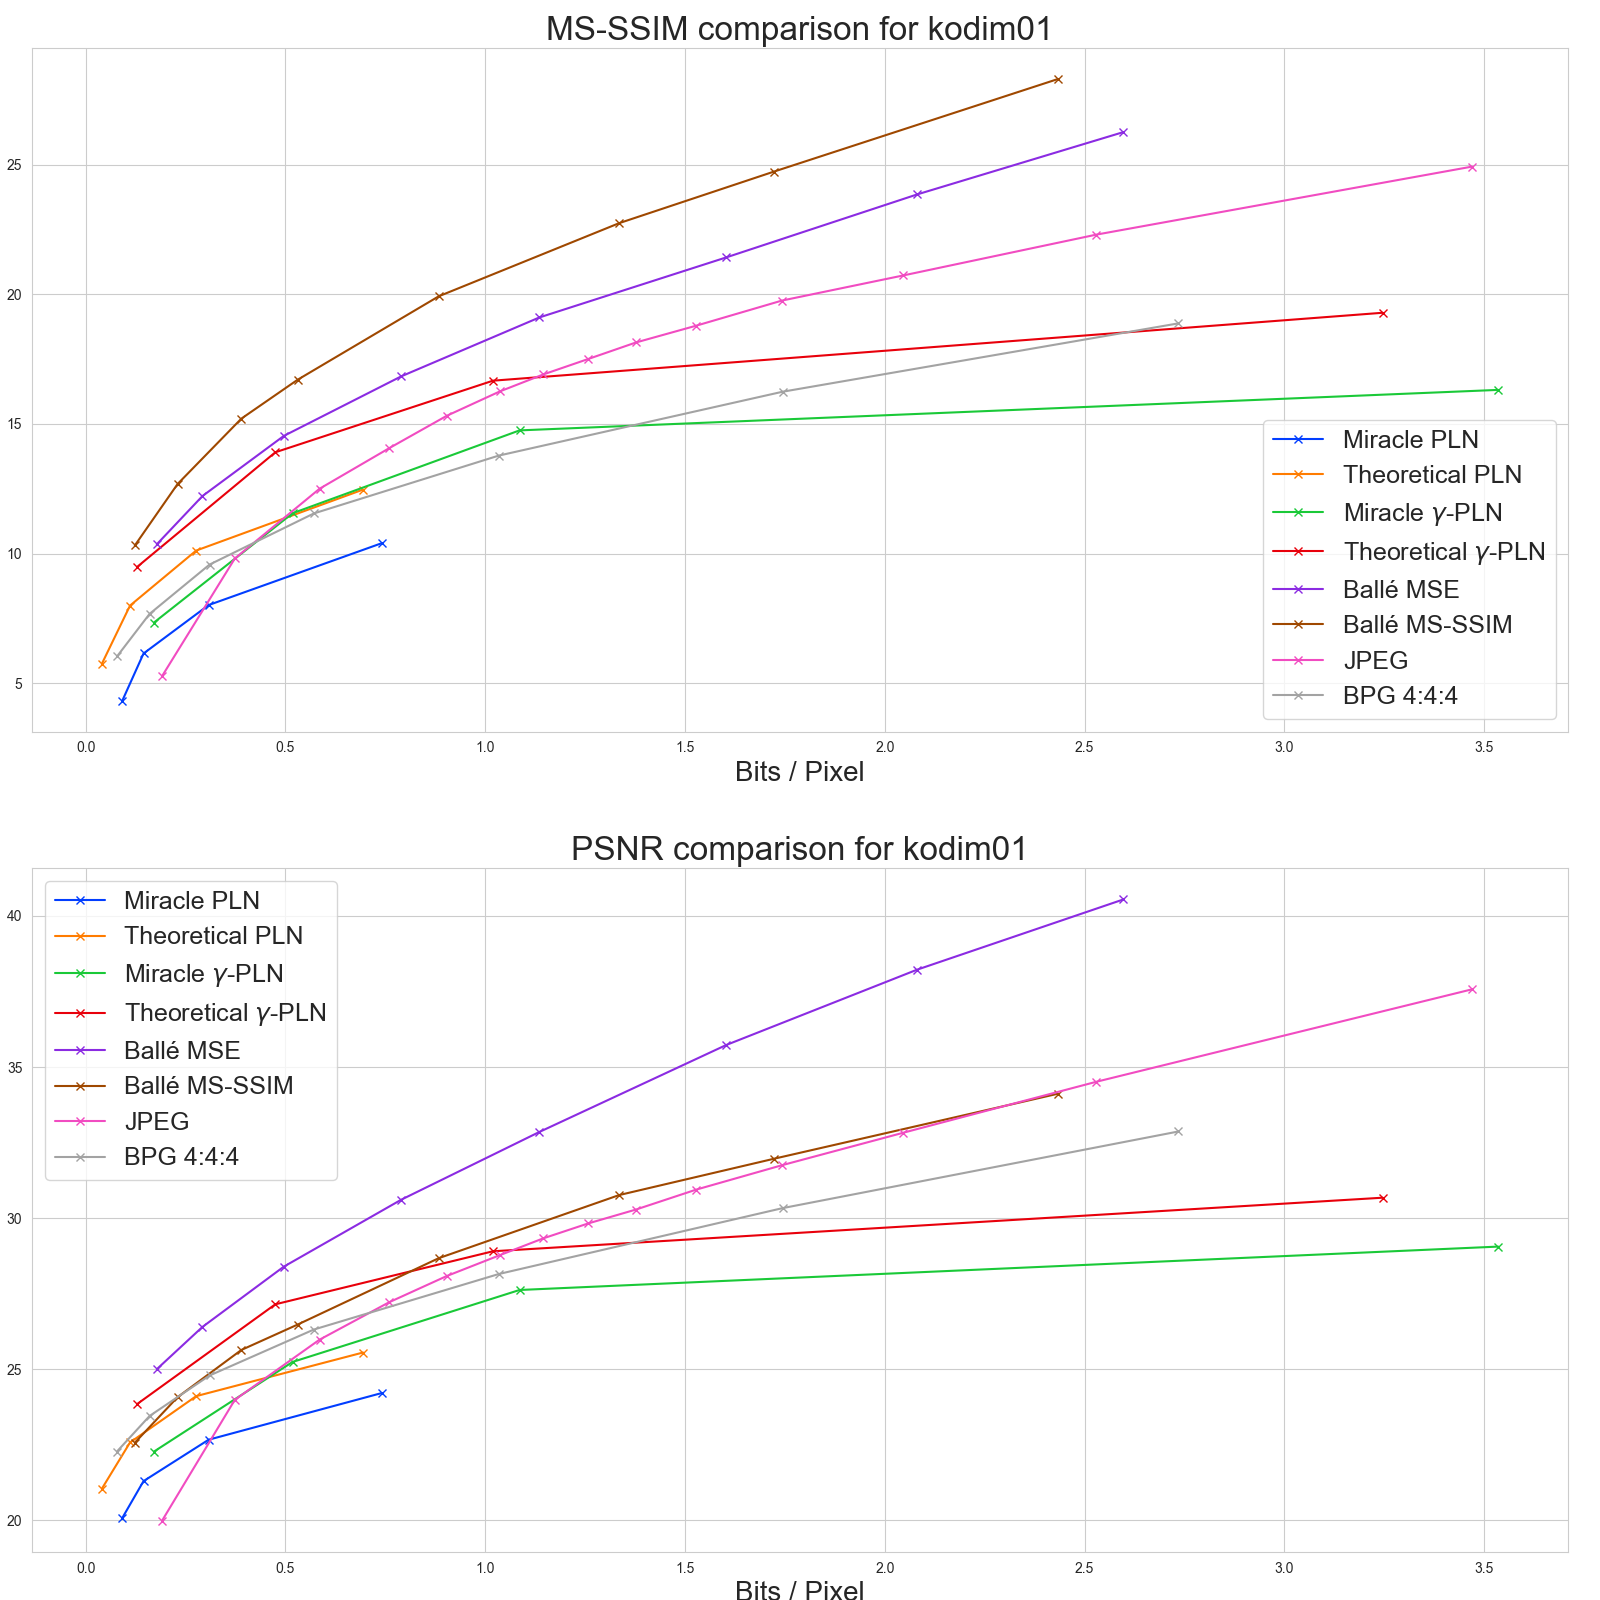
\includegraphics[width=\textwidth]{../img/plots/kodak_comparison/kodim01_comparison}
  \caption{haha}
  \label{fig:kodim01_comp}
\end{figure}
\section{Discussion}
\section{Conclusion}

\cite{townsend2019practical}
\printbibliography

\newpage

\section*{Appendix A: Sampling algorithms}
\subsection*{Rejection Sampling}
\par
The rejection sampling algorithm presented here is due to
\cite{harsha2007communication}.

\begin{algorithm}
  \caption{Rejection sampling presented in \cite{harsha2007communication}.}
  \label{alg:harsha_rej_sampling}
  \begin{algorithmic}[1]
    \Procedure{Rej-Sampler}{$P, Q, \langle x_i \sim Q \mid i \in \Nats \rangle$}
    \Comment $P$ is the prior
    \Statex
    \Comment $Q$ is the posterior
    \Statex
    \Comment $x_i$ are i.i.d. samples from $Q$
    \State $p_0(x) \gets 0 \quad \forall x \in \X$.
    \State $p_0^* \gets 0$.
    \For{$i \gets 1, \hdots \infty$}

    \State
    $\alpha_i(x) \gets \min{P(x) - p_{i - 1}(x), (1 - p_{i - 1}^*)Q(x)}\quad
    \forall x \in \X$

    \State $p_i(x) \gets p_{i - 1}(x) + \alpha_i(x)$
    
    \State $p_i^* \gets \sum_{x \in \X}p_i(x)$

    \State $\beta_i(x_i) \gets \frac{\alpha_i(x)}{(1 - p_i^*)Q(x)}$

    \State Draw $u \sim \Unif{0, 1}$

    \Statex

    \If{$u < \beta_i(x_i)$}

    \State\Return $i, x_i$

    \EndIf
    
    \EndFor
    \EndProcedure
  \end{algorithmic}
\end{algorithm}

\begin{algorithm}
  \caption{Importance sampling algorithm proposed by \cite{havasi2018minimal}}
  \label{alg:miracle_imp_samp}
  \begin{algorithmic}
    \Procedure{Importance-Sampler}{$P, Q, \langle x_i \sim Q \mid i \in \Nats \rangle$}
    \Comment $P$ is the prior
    \Statex
    \Comment $Q$ is the posterior
    \Statex
    \Comment $x_i$ are i.i.d. samples from $Q$

    \State $K \gets \exp\{\KL{Q}{P}\}$

    \State $\tilde{w}_i \gets \frac{Q(x_i)}{P(x_i)} \quad \forall i =
    1,\hdots K$

    \State Sample $j \sim p(\tilde{w})$

    \Return $j, x_j$
    \Statex
    \EndProcedure
  \end{algorithmic}
\end{algorithm}
\section*{Appendix B: Images}
\end{document}